\section{Results}
\label{sec:results}

\subsection{Checks of the theory and of the numerical pipeline}
\label{sec:theory_checks}

\begin{table*}
\caption{Checks of the theory and of the numerical pipeline. The benchmark consists of hard-tanh networks whose fixed
points are enumerated over all $3^N$ linear regions. Copies are model equilibria within $1\%$ of the half-width of the
region $Q$ (half of its largest edge) from a true equilibrium. For the test in the unstable subspace the reference is the ball test of the full protocol;
the last row counts the $27$ networks in which $32$ random directions missed a self-excited attractor.}
\label{tab:theory}
\begin{ruledtabular}
\begin{tabular}{llll}
Result & Check & Data & Count \\
\hline
Thm.~\ref{thm:degree} & Index sum $1$ & hard-tanh benchmark, exact sets & 754/754 \\
 &  & tanh echo state networks & 997/1004 (7 with even $K$) \\
 &  & one-layer / two-layer perceptrons & 3358/3360 / 3279/3360 \\
 &  & residual networks (theorem not applicable) & 1571/3360 \\
Cor.~\ref{cor:counts} & $U\ge(K-1)/2$ & all models with index sum $1$ & no violation \\
 & Incomplete set flagged & Newton sets of the benchmark & 40/43; 0 false of 711 \\
Prop.~\ref{prop:forced} & Copy has index $\iota_j$ & copies within $1\%$ ($0.1\%$) & 440/474 (334/340) \\
 & Chua~I ($s=-1$): copies of all three & echo state networks; mlp; mlp2; res & 0/96; 0/480; 0/480; 23/480 \\
 & Li--Sprott ($s=0$): $K\ge1$ & echo state networks & 32/32 \\
 & Li--Sprott: reproduced, self-excited & training attractor; unseen torus & 29/29; 0/4 \\
Prop.~\ref{prop:manifold} & Test in $E^u$ & self-excited attractors, benchmark & 884/913 \\
 &  & 32 / 256 / 2048 directions, hard cases & 48 / 60 / 70 of 77 \\
\end{tabular}
\end{ruledtabular}
\end{table*}


\begin{figure}
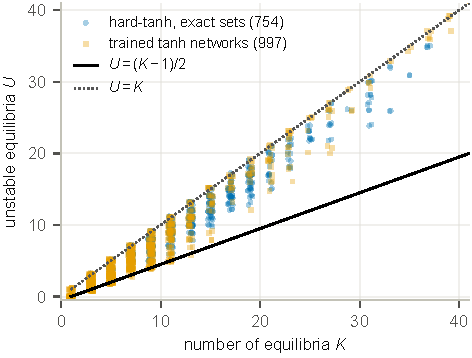
\includegraphics[width=\columnwidth]{figures/fig_theory.pdf}
\caption{Index bookkeeping. Number of unstable equilibria $U$ against the number of equilibria $K$ for the $754$ hard-tanh
benchmark networks with exhaustively enumerated fixed points and the $997$ trained tanh echo state networks of the
full-protocol ensemble (Table~\ref{tab:ensembles}) with index sum $1$; small jitter added. All points lie between the bound
$U=(K-1)/2$ of Corollary~\ref{cor:counts} and $U=K$, and $K$ is always odd.}
\label{fig:theory}
\end{figure}

The theorems need no numerical confirmation; Table~\ref{tab:theory} uses them to validate the numerical pipeline. On the
$754$ hard-tanh benchmark networks ($N=8$--$20$, $K$ between $3$ and $37$), the enumerated indices sum to $1$ in every
network and $K$ is always odd. Among the $1004$ trained tanh echo state networks of the full-protocol ensemble, $997$ have
index sum $1$; the other seven are exactly those with an even number of found equilibria, so their sets are incomplete. The
index sum is $1$ in $3358$ of the $3360$ one-layer and $3279$ of the $3360$ two-layer perceptrons; $76$ of the $81$ two-layer
exceptions have width $512$ or $1024$ and tens to hundreds of equilibria. No network or model with index sum $1$ violates
$U\ge(K-1)/2$ (Fig.~\ref{fig:theory}), and the indices computed from the Jacobians agree with Lemma~\ref{lem:parity} at
all $18\,019$ fixed points of the benchmark and the trained echo state networks, a check of the Jacobians themselves. Residual networks, to which Theorem~\ref{thm:degree} does not apply, have index sum $1$ in
$47\%$ of the cases. Newton's method from the standard starting points missed equilibria in $43$ benchmark networks; in $40$
of them the index sum of the found set differs from $1$, the three sets that pass the check each miss a pair of
equilibria of opposite index, and there are no false alarms.

Two further checks address sets that pass this test and still miss equilibria (supplementary material). For $184$ echo
state networks of the six regimes, rebuilt from the size sweep and from the full-protocol ensemble at $\rho=1.2$, repeating
the search with four ($N\ge700$) or eight ($N\le300$) times as many Newton starts found no further equilibrium in any of the
$136$ networks with $\rho=0.9$, up to $N=2000$ with $33$ unstable equilibria per network on average, and one further unstable
equilibrium in two of the $48$ networks with $\rho=1.2$, neither of which reproduces the hidden attractor; no attractor that
was not excited became excited. In the full-protocol ensemble the $6.8\times10^6$ Newton runs started near the basin
boundaries of candidate hidden attractors found no new equilibrium. For the perceptrons and residual networks we retrained
$960$ models with saved weights, $720$ of them identical to models of Sec.~\ref{sec:classes}, and enumerated their fixed
points by the interval Krawczyk method,\cite{Krawczyk1969Newton,Moore2009Interval} which certifies all fixed points in a box
that contains every fixed point of a bounded model (for residual networks, in $Q$). In every model the certified set equals
the set found by Newton's method.

The forced equilibria of Proposition~\ref{prop:forced} appear where $s\neq1$. An equilibrium of an echo state network that
lies within $1\%$ of the half-width of the region from a true equilibrium (a copy, in what follows) has the index $\iota_j$
of that equilibrium in $440$ of $474$ cases, and in $334$ of the $340$ cases closer than $0.1\%$. The sufficient condition of
Proposition~\ref{prop:forced} cannot be checked directly for trained models; this agreement of indices is the empirical
evidence for its conclusion. The intervention ensemble of Sec.~\ref{sec:data_effects}, whose readout imposes the true
equilibria as exact equilibria of the network, illustrates the bookkeeping: all $66$ networks have index sum $1$ and all
imposed copies, but the copies carry the true indices in only about half of them ($5$ of $16$ in Chua~I), since imposing
the location of an equilibrium does not impose its type (the imposed origin of Chua~I is stable in none of the $16$). Where
they do, the remaining equilibria have total index $1-s$; in Chua~I this forces at least two of them, and these networks
have on average $3.2$, $1.6$ of them stable. For Chua~I ($s=-1$), none of the $96$ echo state
networks and none of the $960$ one- and two-layer perceptrons has copies of all three true equilibria, whereas the
unbounded residual networks have them in $23$ of $480$ cases; the bounded models that copy two of the three (the origin and
one saddle-focus) have spurious equilibria of total index $+1$, on average $2.2$ of them, $1.4$ stable. For the
equilibrium-free Li--Sprott system ($s=0$) every one of the $32$ echo state networks has at least one equilibrium, and all
of these equilibria are unstable. The training attractor, hidden in the true system, is reproduced $29$ times and is
self-excited from these forced equilibria in all $29$; the unseen torus, reproduced in four networks as in the experiment of
R\"ohm \textit{et al.},\cite{Rohm2021} is statistically hidden in all four.

The excitation test in the unstable subspace (Sec.~\ref{sec:manifold}) is efficient but not exhaustive. On the benchmark it
samples the basis directions of $E^u$ and $32$ random directions in it, $37$ points per equilibrium and radius on average
instead of the $1000$ of the reference ball, and finds $884$ of the $913$ self-excited attractors. Once it excites an
attractor that the full protocol had labeled statistically hidden, which shows that a statistically hidden label can be
wrong (one of $46$ on the benchmark). In the $27$ networks with misses, the number of self-excited attractors found grows
from $48$ of $77$ with $32$ directions to $60$ with $256$ and $70$ with $2048$; the seven never found are limit cycles of
networks whose equilibria have unstable subspaces of dimension up to $9$, and whose basins are reached from a tiny
fraction of the directions.

\subsection{Survival law in echo state networks}
\label{sec:esn_law}

\begin{figure*}
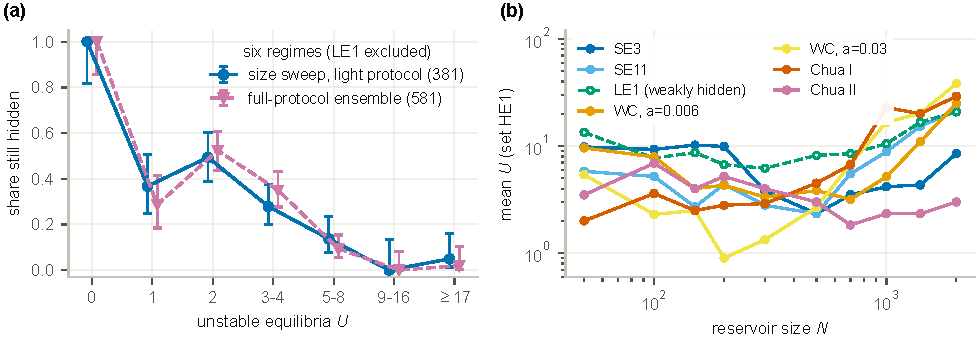
\includegraphics[width=\textwidth]{figures/fig_esn_law.pdf}
\caption{Survival law in echo state networks. (a) Share of reproduced hidden attractors that are not excited from any
unstable equilibrium of the network, against the number $U$ of unstable equilibria, with Wilson $95\%$ intervals; the legend
gives the number of rows; six regimes, LE1 excluded. Solid: size sweep ($620$ networks with $N=50$--$2000$,
Table~\ref{tab:ensembles}), one row per
pair (network, attractor), labeled by the light protocol (balls of radii $10^{-6}$, $10^{-4}$ and $10^{-3}$ around each
unstable equilibrium); dashed: full-protocol ensemble, one row per network, share labeled statistically hidden (not
excited at any radius up to $10^{-1}$, with a bound of at most $0.05$ on the chance that an exciting equilibrium was
missed; Sec.~\ref{sec:protocol}). (b) Mean $U$ against reservoir size for the networks trained on HE1 (the hidden
trajectory plus $20$ transients toward the visible attractor), one line per regime; LE1 dashed.}
\label{fig:esn_law}
\end{figure*}

Figure~\ref{fig:esn_law} shows the survival of reproduced hidden attractors in the size sweep, pooled over the six regimes
whose attractors are hidden in the strict sense: $620$ networks, $776$ pairs (network, hidden attractor), of which $381$ have
the attractor reproduced and index sum $1$. At $U=0$ the attractor is not excited in all $17$ pairs; this point carries no
information beyond the completeness of the equilibrium set, since by Corollary~\ref{cor:criterion} an attractor cannot be
excited without unstable equilibria. One unstable equilibrium brings the share down to $0.37$ $[0.25, 0.51]$, and it
decreases further to $0.14$ at $U=5$--$8$ and $0.05$ at $U\ge17$. The share at $U=2$, $0.49$, exceeds that at $U=1$ because
of the regime mix: $30$ of the $49$ pairs with $U=1$ come from the two Wang--Chen regimes, where none survives, and in no
regime is survival at $U=2$ higher than at $U=1$ (Mantel--Haenszel odds ratio $0.04$ $[0.003, 0.47]$); standardized to
a common regime mix, the shares are $0.60$ $[0.49,0.68]$ at $U=1$ and $0.45$ $[0.38,0.52]$ at $U=2$ (supplementary
material). In a logistic regression with regime fixed effects and terms for the training set and the network size, the
coefficient of $\log(1+U)$ is $-3.08\pm0.40$ (cluster-bootstrap $95\%$ interval $[-4.9,-2.0]$, $380$ networks;
likelihood-ratio $\chi^2=123$), and the decline does not rest on the step from $U=0$: on pairs with $U\ge1$ the coefficient
is $-2.40\pm0.39$. With LE1 added it is $-3.26\pm0.40$. Among links and transformations of $U$, the logit in $\log(1+U)$
has the lowest AIC, and the result is unchanged when the thresholds that define a reproduction are moved from $0.2$ to
$0.1$ or $0.3$ ($-3.25$, $-3.08$). The
network size adds no detectable effect beyond $U$: the coefficient of $\log N$ is $-0.03\pm0.18$ (likelihood-ratio
$p=0.86$), although its $95\%$ interval still allows a change of the log-odds between $-1.7$ and $+1.5$ over the range of
$N$. Size acts mainly through the number of unstable equilibria it produces, which is not monotone in $N$
(Table~\ref{tab:UN}): it grows overall with $N$ for Chua~I, from $2$ at $N=50$ to $29$ at $N=2000$, and has a minimum at
intermediate sizes, between $N=200$ and $700$, for the other regimes trained on HE1.

Two further checks give the same shape. In the full-protocol ensemble, the $581$ networks that reproduce a hidden attractor
(one row per network) keep it statistically hidden in $23$ of $23$ cases at $U=0$, in $0.29$, $0.52$ and $0.35$ of the cases at
$U=1$, $2$ and $3$--$4$ (the same regime mix inverts the first two), in $0.09$ at $U=5$--$8$ and in one of $94$ at $U\ge9$.
Counted by $\Uin$, the unstable equilibria whose physical image $W_{\mathrm{out}}r^*$ lies in $Q$, the decline is monotone:
$0.96$, $0.41$, $0.35$, $0.25$ and $0.03$ at $\Uin=0$, $1$, $2$, $3$--$4$ and $5$--$8$. The coefficient of $\log(1+\Uin)$
is $-3.54\pm0.35$, against $-4.25\pm0.42$ for $\log(1+U)$, and the equilibria outside $Q$ add a smaller effect
($-1.9\pm0.8$); for echo state networks, whose state space is the reservoir, we keep $U$ as the main count. The excitation
came from spurious equilibria alone in $93\%$ of the losses of hiddenness ($383$ of $412$), and from a copy of a true
equilibrium in the rest; the share is $86$--$95\%$ when the distance that defines a copy is halved or doubled. The settings
sweep (SE3, SE11 and Chua~I, $121$ pairs) varies the input scale and the reservoir density and gives a similar coefficient,
$-3.32\pm0.77$; here the settings add an effect beyond $U$ ($\chi^2=17.0$, four degrees of freedom, $p=0.002$), with
coefficients of about $+2$ for the sparser reservoir and for both changed input scales.

The reference curve~\eqref{eq:heuristic} with two branches gives the order of the decay but not its details when $p_B$ is
the basin fraction measured in each network, the share of uniform points of the reservoir cube $[-1,1]^N$ that reach the
reproduced attractor; this is not the $p_B$ of the true system in Table~\ref{tab:systems}. Fitting $\Pr(\text{hidden}\mid U)=q^U$ by maximum likelihood gives $q=0.77$, $0.85$ and
$0.78$ for Chua~I, LE1 and SE3, within $0.03$ of $(1-p_B)^2=0.78$, $0.87$ and $0.81$. For the Wang--Chen system at $a=0.006$,
whose hidden attractor attracts about two thirds of the region, $(1-p_B)^2=0.10$ and the fitted $q$ is close to zero. For SE11
($0.83$ against $0.94$), the cycle of Wang--Chen at $a=0.03$ ($0.18$ against $0.33$) and Chua~II ($0.73$ against $0.99$, $13$
pairs) the observed survival is lower than predicted. Across regimes the heuristic fails as a law: the slopes differ
significantly between regimes (interaction with $\log(1+U)$: likelihood ratio $23$, five degrees of freedom, $p=3\times10^{-4}$),
but by a factor of about two, whereas $\log(1-p_B)$ varies over two orders of magnitude, and a common $\nu$ is rejected.
Survival depends on $U$ in a similar way whether the attractor fills a large or a tiny part of the cube. Equilibria are not
random points of the region, and Sec.~\ref{sec:classes} quantifies how they differ.

\subsection{A similar decline across model classes}
\label{sec:classes}

\begin{table}
\caption{Survival of reproduced hidden attractors: share not excited from any unstable equilibrium, with the number of
pairs (model, hidden attractor) in parentheses, by the number of unstable equilibria: all of them ($U$) for echo state
networks (ESN), those in the region ($\Uin$) for the other classes. ESN: size sweep (Table~\ref{tab:ensembles}); the last
row merges the bins $9$--$16$ and $\ge17$ of Fig.~\ref{fig:esn_law}. Perceptrons (mlp, mlp2) and residual networks (res):
all training sets (H1, E1, HE1; Sec.~\ref{sec:data}). Light protocol (Sec.~\ref{sec:protocol}). Pooled over the six regimes
with strictly hidden attractors; LE1 is reported separately (Sec.~\ref{sec:systems}).}
\label{tab:classes}
\begin{ruledtabular}
\begin{tabular}{lcccc}
$U$ or $\Uin$ & ESN & mlp & mlp2 & res \\
\hline
$0$ & 1.00 (17) & 0.99 (426) & 0.99 (268) & 0.80 (264) \\
$1$ & 0.37 (49) & 0.32 (421) & 0.26 (405) & 0.30 (347) \\
$2$ & 0.49 (79) & 0.18 (154) & 0.28 (130) & 0.28 (286) \\
$3$--$4$ & 0.28 (97) & 0.07 (70) & 0.10 (171) & 0.18 (155) \\
$5$--$8$ & 0.14 (73) & 0.00 (2) & 0.06 (105) & 0.08 (26) \\
$\ge9$ & 0.03 (66) & -- & 0.01 (98) & 0.00 (1) \\
\end{tabular}
\end{ruledtabular}
\end{table}


\begin{figure*}
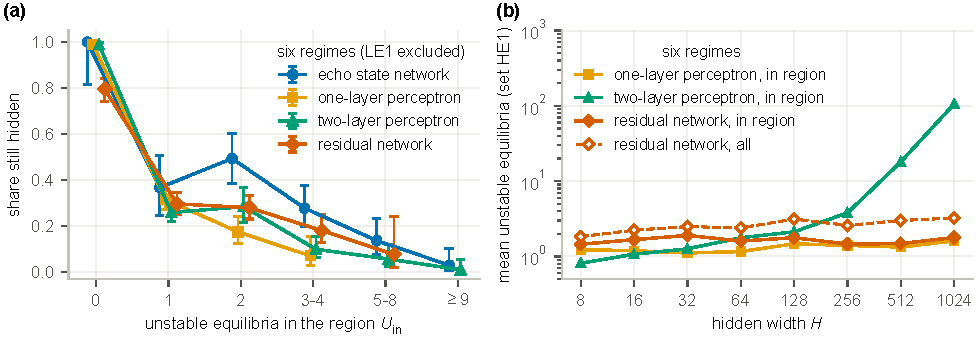
\includegraphics[width=\textwidth]{figures/fig_classes.pdf}
\caption{Survival across model classes. (a) Share of reproduced hidden attractors that stay hidden against the number of
unstable equilibria in the region of the true system, for echo state networks (size sweep, all equilibria counted) and for
one-layer perceptrons, two-layer perceptrons and residual networks (training sets H1, the hidden trajectory; E1, $20$
transients toward the visible attractor; HE1, both); six regimes, LE1 excluded; light protocol, Wilson $95\%$ intervals,
points with fewer than $5$ pairs omitted. (b) Mean number of unstable equilibria against hidden width for models trained on HE1: inside the region
(solid) and, for residual networks, in total (dashed, open symbols).}
\label{fig:classes}
\end{figure*}

The perceptrons and residual networks trained on H1 and HE1 reproduce the hidden attractors in a third to a half of the
cases and lose hiddenness in a similar way (Fig.~\ref{fig:classes}, Table~\ref{tab:classes}). With $\Uin$ counted inside the
region of the true system, the share of attractors that stay hidden falls from $0.99$ at $\Uin=0$ for both perceptrons
($0.80$ for residual networks, whose unstable equilibria outside the region can still excite the attractor) to
$0.26$--$0.32$ at $\Uin=1$ in every class, and to $0.06$ and $0.08$ at $\Uin=5$--$8$ for the two classes that reach these
values. In a logistic regression on the $3329$ reproduced pairs with regime effects, the coefficient of $\log(1+\Uin)$ is
$-3.94\pm0.15$ ($\pm0.24$ with errors clustered by training group of $20$ seeds; cluster-bootstrap interval over the
$3284$ models $[-4.27,-3.67]$; $-3.36\pm0.12$ with LE1). The slope differs between regimes ($p<10^{-6}$), from $-2.7$
in SE11 to $-5.4$ in Wang--Chen at $a=0.006$. Additive class terms are small but not negligible:
$-0.36\pm0.13$ for two-layer perceptrons and $-0.15\pm0.12$ for residual networks ($p=0.002$ for the class). The hidden width
has an effect of $-0.14\pm0.03$ per unit of $\log H$ ($\pm0.07$ cluster-robust). The coefficient of $\log(1+\Uin)$ is
unchanged by terms for the quality of the fit ($\Delta_{\mathrm{att}}$, $d_H$ and training error, $-3.95$), by restricting
to complete equilibrium sets ($-3.94$), by counting attractors excited only at a finite radius as hidden ($-3.88$; there
are $14$ such pairs), by moving the reproduction thresholds to $0.1$ or $0.3$ ($-3.69$, $-4.06$) and by enlarging $Q$ by a
factor of up to two ($-4.06$); halving $Q$ drops equilibria of its outer part and weakens it to $-2.74$. On pairs with
$\Uin\ge1$ it is $-2.74\pm0.22$. The classes are not identical, however: a model with class-specific slopes fits
better (likelihood ratio $82$, two degrees of freedom), with slopes $-5.8$, $-4.1$ and $-2.8$ for one-layer perceptrons,
two-layer perceptrons and residual networks. In a joint fit, echo state networks (slope $-2.2\pm0.3$, counted by $U$)
decline more slowly than both perceptrons and about as fast as residual networks. The class acts mainly, not only,
through $\Uin$.

The classes differ most in how many unstable equilibria they produce. A one-layer perceptron trained on HE1 has on average
$1.1$--$1.6$ unstable equilibria in the region at every width. A two-layer perceptron trained on HE1 has $0.8$ at width $8$,
$3.8$ at width $256$, $18$ at $512$ and $106$ at $1024$; trained on H1, it keeps a reproduced attractor hidden less often
than a one-layer perceptron ($0.28$ against $0.47$). Depth harms hiddenness mainly by creating equilibria. Residual networks have $1.8$ to $3.2$ unstable equilibria on
average, of which $1.5$--$1.9$ lie in the region; counting the others would move them off the common curve. Unstable
equilibria outside the region are not harmless, though: they excite the reproduced attractor in $36\%$ of the cases, which
explains why residual networks keep hiddenness at $\Uin=0$ in only $0.80$ of the cases.

Single equilibria show what the counts hide. An unstable equilibrium inside the region excites the reproduced attractor in
$62\%$ of the cases, against $48\%$ for points of the region at the same distance from the attractor that lie in its basin;
the excess is large in Chua's circuit and SE11 and absent for perceptrons in the Wang--Chen regimes and SE3. Excitation
falls with the distance to the attractor, from $0.88$ within $0.03$ of its diameter to $0.28$ beyond one diameter, and
$77\%$ of the exciting equilibria send part of a small ball elsewhere, as equilibria on a basin boundary
(Corollary~\ref{cor:criterion}) do. Spurious equilibria excite in $63\%$ of the cases, whatever the distance that defines a
copy. Copies of the true saddle-foci of Chua's circuit excite in $68\%$ ($111$ of $164$), although the true saddle-foci do
not: a locally faithful copy does not carry a faithful unstable manifold. Unstable copies of true stable equilibria excite
in $30\%$. Equilibria with one, two and three unstable directions excite in $55\%$, $66\%$ and $66\%$, and unstable foci
excite more often than saddles ($0.67$ against $0.55$). A real eigenvalue below $-1$, which has no counterpart in the flow map of the
true system (its real eigenvalues $e^{h\lambda}$ are positive), is rare: it is the only unstable direction of $51$ of the
$2951$ equilibria with one unstable direction (index $+1$ instead of $-1$), and these excite in $27\%$ of the cases, against
$55\%$ for an eigenvalue above $1$; another $245$ equilibria combine one eigenvalue above $1$ with one below $-1$. If the
equilibria of a model excited the attractor independently with these probabilities, survival would be $0.09$ at
$\Uin=3$--$4$ and $0.03$ at $\Uin=5$--$8$; the observed values are $0.13$ and $0.06$. Excitation is correlated within a
model: in a logistic model of single equilibria with a random effect per model, the latent intra-model correlation is
$0.48$ (median odds ratio $5.2$; likelihood ratio against no random effect $1095$), the population-averaged probability that
an equilibrium inside $Q$ excites the attractor is $0.68$, and this model reproduces the survival curve, which independent
equilibria underpredict. Some models place all their equilibria so that none reaches the basin. In LE1, whose attractor is reached in the true system from a segment of the unstable half-line
of equilibria (Sec.~\ref{sec:systems}), copies of the line excite the reproduced attractor in $16\%$ of the cases and
spurious equilibria in $61\%$, and survival stays at $0.35$--$0.47$ for $\Uin\ge3$: a model that copies the line keeps
part of its weak hiddenness.

\subsection{What the data do}
\label{sec:data_effects}

\begin{figure}
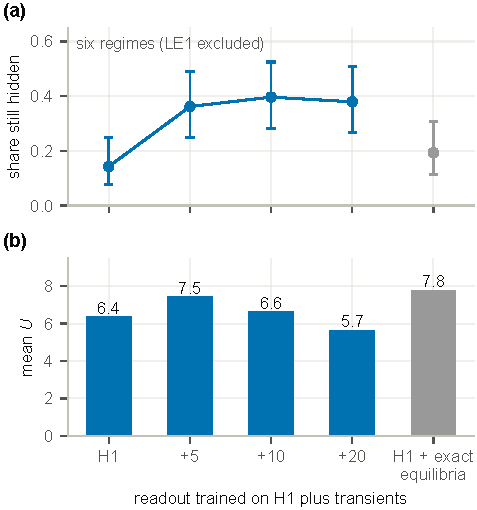
\includegraphics[width=\columnwidth]{figures/fig_intervention.pdf}
\caption{Intervention by data: the reservoirs of $66$ echo state networks (six regimes, LE1 excluded) are kept and only the
readout is refitted on
the hidden trajectory H1 plus $0$, $5$, $10$ or $20$ transients toward the visible equilibrium, or on H1 with the true
equilibria imposed as exact equilibria of the network (gray). (a) Share of reproduced hidden attractors that stay hidden
(first hidden attractor of each network), with Wilson $95\%$ intervals. (b) Mean number of unstable equilibria. Survival
rises with five transients and then levels off; the mean $U$ falls in most regimes and rises in Chua~II; imposing the true
equilibria raises $U$. Light protocol.}
\label{fig:intervention}
\end{figure}

The training set is the main factor beyond $U$. Adding the transients of HE1 to the hidden trajectory raises the odds of
survival at fixed $\Uin$ by a factor of $e^{1.52}\approx4.6$ (coefficient $1.52\pm0.20$ with cluster-robust errors). To
separate this effect from $U$, the intervention ensemble keeps the reservoirs of $66$ echo state networks of the six
regimes ($48$ with $N=300$ and $18$ with $N=700$) and refits only the readout on H1 with $0$, $5$, $10$ or $20$ added
transients (Fig.~\ref{fig:intervention}). The share of reproduced attractors that stay hidden rises from $0.14$
$[0.08, 0.25]$ on H1 to $0.36$, $0.40$ and $0.38$ $[0.27, 0.51]$ with $5$, $10$ and $20$ transients: five transients give
the whole effect. Within a network, going from H1 to E20 lowers $U$ in $38$ of $55$ pairs; hiddenness appears in $17$
pairs, $15$ of them with fewer unstable equilibria and two with the same number, and is lost in three.

In the echo state networks the transients act largely, but not only, through $U$. Within a network, $U$ falls in $33$, $38$
and $38$ of the $55$--$56$ pairs from H1 to E5, E10 and E20, and of the $15$, $18$ and $17$ pairs in which hiddenness appears,
only one has more unstable equilibria. A mediation analysis through $\log(1+U)$ with cluster-bootstrap intervals attributes
$54\%$ $[33,91]$, $61\%$ $[40,100]$ and $77\%$ $[51,129]$ of the effect of E5, E10 and E20 to the change of $U$; the direct
effect is borderline for E5 and E10 and not significant for E20. In a regression on the five described variants with regime
effects and $\log N$, the coefficient of E20 is $1.6\pm0.5$ without and $0.9\pm0.6$ with $\log(1+U)$, whose own coefficient
is $-3.74\pm0.58$. The mean $U$ over all networks rises with five transients ($6.4$ to $7.5$, Fig.~\ref{fig:intervention})
only because it rises by about $29$ in Chua~II, whose networks reproduce nothing on these sets; it falls in Chua~I ($9.9$ to
$3.8$ with E20), SE11 ($6.1$ to $2.6$) and Wang--Chen at $a=0.03$. The transients also shrink the basin of the reproduced
attractor, in all five regimes with reproductions on E20 (Chua~I from $0.22$ to $0.13$ of the reservoir cube). In LE1 the
transients act differently: the share of unstable equilibria that excite the attractor drops from $0.53$ to $0.01$ while
their number grows from $4.8$ to $6.6$, and survival rises from $3$ to $14$ of $16$, far above what
Eq.~\eqref{eq:heuristic} predicts from the changes of $U$ and $p_B$. Constraining the readout so that the true equilibria
become exact equilibria of the network ($W_{\mathrm{out}}r^*=x^*$) raises $U$ in $40$ of the $66$ networks (Chua~I from
$9.9$ to $13.3$) and leaves survival almost unchanged ($0.19$); its positive effect at fixed $U$ ($+1.5\pm0.6$) is offset by
the additional unstable equilibria.

\subsection{Changing U at fixed data}
\label{sec:penalty}

The survival law is observational: $\Uin$ varies with the class, the width and the seed, and something else could vary with
it. The penalty experiment changes $\Uin$ at fixed data, class and seed. Two-layer perceptrons ($H=256$) were trained on H1
and HE1 in the six regimes with a term in the loss that pushes the spectral radius of every equilibrium found in $Q$ below
one, with weight $\lambda_{\mathrm{P}}=0$, $0.1$ or $1$ and the same seeds and minibatches in the three arms ($720$ models,
Appendix~\ref{app:training}). The penalty removes unstable equilibria at an unchanged one-step error: the mean $\Uin$ falls
from $2.70$ to $0.05$ and $0.11$, it decreases in $88\%$ of the paired models and increases in at most $3$ of the $240$, and
the median ratio of the one-step training errors to the unpenalized ones is $0.92$ and $0.99$ (at $\lambda_{\mathrm{P}}=1$ a tenth of the
models fit $2.3$ times worse or more). It removes them indiscriminately, however: in Chua's circuit, whose true unstable
equilibria lie in $Q$, the penalized models have almost none, so they cannot reproduce the true equilibrium structure there. Reproduction drops
from $195$ to $170$ and $162$ of the $320$ pairs (model, hidden attractor), mostly in Chua~II and SE11. Among the reproduced
attractors the share that stays hidden rises from $0.27$ $[0.21,0.34]$ to $0.994$ $[0.97,1.00]$ at both values of $\lambda_{\mathrm{P}}$,
so the number of hidden reproductions triples ($53$, $169$ and $161$). Of the $150$ pairs reproduced both without the
penalty and with $\lambda_{\mathrm{P}}=0.1$, the attractor became hidden in $114$ and lost hiddenness in one (McNemar $p<10^{-32}$).

The penalty acts mainly by moving the models to $\Uin=0$. Of the $332$ penalized reproductions, $325$ have $\Uin=0$, and all
of them keep the attractor hidden. Two-layer perceptrons of the model-class ensemble with the same regime, training set
and $\Uin$ would keep it hidden in $166.5$ of the $170$ penalized reproductions at $\lambda_{\mathrm{P}}=0.1$ and in $157.7$ of
the $162$ at $\lambda_{\mathrm{P}}=1$; $169$ and $161$ are observed (exact $p=0.10$ and $0.05$), so the penalty adds at most
a marginal effect beyond $\Uin$. In a logistic regression on the $527$ reproduced pairs with regime and training-set effects, $\log(1+\Uin)$ and
a step at $\Uin=0$, indicators of $\lambda_{\mathrm{P}}$ add nothing ($\chi^2=0.22$, two degrees of freedom, $p=0.90$), but this test has
little power: the step term is almost separated, and only seven penalized reproductions keep $\Uin\ge1$. The experiment
therefore tests the step from $\Uin\ge1$ to $\Uin=0$, not the curve beyond it. The unstable equilibria that survive the
penalty are nearly neutral (largest spectral radius below $1.05$ in five of the seven), and such equilibria rarely excite
the attractor even without the penalty: at $\lambda_{\mathrm{P}}=0$, models whose unstable equilibria in $Q$ all have a spectral radius below $1.05$ keep it
hidden in $9$ of $11$ cases, against $24$ of $164$ otherwise. Survival depends also on how unstable the equilibria are;
their number is the main variable but not the only one.

The penalty removes saddles by annihilation, not by pushing them out of $Q$: of the $292$ equilibria of index $-1$ inside
$Q$ without the penalty, $285$ and $272$ are gone at $\lambda_{\mathrm{P}}=0.1$ and $1$, the total number of equilibria falls
from $826$ to $260$ and $294$, and the penalized reproductions have no unstable equilibria outside $Q$. Its effect on the
fidelity of the model depends on the data (Sec.~\ref{sec:fidelity}). On HE1 the penalized models keep a stable copy of the
visible equilibrium (all of them, against $78\%$ without the penalty) and are hidden and faithful in $0.64$ of the
reproductions instead of $0.10$; on H1 they hide the attractor without having the visible equilibrium. The share of the true
hidden basin that reaches the reproduced attractor falls, from $0.81$ to $0.73$ at $\lambda_{\mathrm{P}}=0.1$ and from
$0.75$ to $0.54$ at $\lambda_{\mathrm{P}}=1$, and the penalty deletes the copies of the saddle-focus of Chua~II.

In LE1 the penalty makes the model more hidden than the true system: the true attractor is reached from a segment of the
unstable half-line of equilibria (Sec.~\ref{sec:systems}), while the penalized models keep it hidden in all $59$
reproductions, against $17$ of $34$ without the penalty; their remaining unstable equilibria are all nearly neutral. The
penalty is a prior on the equilibria rather than something learned from the data, and it makes the model faithful only
where the true system has no unstable equilibria in $Q$.

\subsection{Hidden is not faithful}
\label{sec:fidelity}

Survival is measured with respect to the model's own equilibria and says nothing about whether the model is right
elsewhere. Three measures that do not depend on these equilibria compare each model with the true system on the uniform
points of $Q$ (supplementary material): the share of points whose outcome in the model corresponds to the true one,
counted over the points that stay bounded in the true system; the share of the true hidden basin that reaches the
reproduced attractor; and whether the model has a stable copy of the visible equilibrium. We call a reproduction faithful
if the model has this copy, at least half of the true hidden basin reaches the reproduced attractor, and the model basin,
restricted to points that stay bounded in the true system, is within a factor of two of the true one.

By these measures survival and fidelity part ways. Models trained on H1, which shows nothing of the visible state, almost
never have a stable copy of the visible equilibrium ($10$ of $800$ one-layer and $3$ of $800$ two-layer perceptrons, $60$ of
$800$ residual networks, $9$ of $278$ echo state networks of the full-protocol ensemble), yet $18$--$34\%$ of their
reproductions stay hidden: there the hidden attractor coexists with spurious stable equilibria, other oscillations or
escape. Of all reproductions by perceptrons and residual networks, $16.5\%$ are hidden and faithful ($27$--$45\%$ on HE1,
under $1\%$ on H1); among echo state networks, $4.6\%$. Within regime, class and training set, the hidden reproductions of
perceptrons and residual networks even have less faithful basins than the excited ones, while for echo state networks they
are slightly more faithful.

The basins of the reproduced attractors are often much too large. In Chua~I the median model basin of one-layer
perceptrons is $0.21$ of $Q$ against $0.020$ per attractor in the true system, but the excess consists of points that escape
to infinity in the true system; on the points that stay bounded, the ratio is close to one. In Chua~II, where nothing
escapes, perceptrons trained on H1 have basins $130$--$160$ times too large, and the transients of HE1 bring them down to a
few times the true size. A model can thus keep a hidden attractor hidden while being far from faithful, and survival is to
be read together with these measures.

\subsection{Training without the hidden attractor}
\label{sec:e1}

\begin{table*}
\caption{Training without the hidden attractor (set E1). Distance: smallest distance from an E1 sample to the hidden
attractor, in units of the attractor's standard deviation per coordinate; coverage: fraction of the attractor within $0.1$
of the E1 data (two values for the two attractors of Chua's circuit). Reproductions are counted over pairs (model, hidden
attractor). Quadratic: sparse quadratic maps fitted by sequential thresholding; NG-RC: next-generation reservoir computer
with the exact quadratic library. LE1, whose attractor is hidden only in a weak sense (Sec.~\ref{sec:systems}), is listed
for completeness.}
\label{tab:e1}
\begin{ruledtabular}
\begin{tabular}{lcccccccc}
Regime & Distance & Coverage & Echo state & mlp & mlp2 & res & Quadratic & NG-RC \\
\hline
SE3 & 0.03 & 0.37 & 1/30 & 5/160 & 0/160 & 3/160 & 0/30 & 23/30 \\
SE11 & 0.11 & 0.00 & 0/19 & 0/160 & 0/160 & 0/160 & 0/30 & 0/30 \\
LE1 & 0.07 & 0.01 & 0/24 & 0/160 & 0/160 & 0/160 & 0/30 & 0/30 \\
WC & 0.55 & 0.00 & 0/18 & 0/160 & 0/160 & 0/160 & 0/30 & 0/30 \\
WC$'$ & 0.40 & 0.00 & 0/18 & 0/160 & 0/160 & 0/160 & 1/30 & 11/30 \\
Chua I & 0.14 / 0.04 & 0.00 / 0.05 & 0/36 & 40/320 & 3/320 & 38/320 & 0/60 & 0/60 \\
Chua II & 1.54 / 1.84 & 0.00 / 0.00 & 0/36 & 0/320 & 1/320 & 0/320 & 0/60 & 0/60 \\
\end{tabular}
\end{ruledtabular}
\end{table*}


Set E1 contains no trajectory on the hidden attractor; it asks whether a model infers the attractor from the transients of
the visible one (Table~\ref{tab:e1}). It does so only where the data nearly show it. In the four regimes where none of
the hidden attractor lies within $0.1$ standard deviations of the E1 data (SE11, both Wang--Chen regimes and Chua~II), one
of the $1920$ perceptrons and residual networks reproduced it. Of the $121$ echo state networks of the six regimes trained
on E1, one reproduced the attractor of SE3, as a self-excited one, and none reproduced any other; in LE1 no model of any
class reproduced it. In SE3 and Chua~I the transients of the visible basin pass along the
attractor itself: in SE3 more than a third of the attractor lies within $0.1$ standard deviations of the E1 data, and in
Chua~I the stable origin attracts so slowly (real part of the eigenvalue $-0.004$) that transients of its basin run beside
the hidden attractor for a long time. There, one-layer perceptrons and residual networks reproduce the attractor in
$2$--$13\%$ of the cases, $69$ of $78$ times the one of the pair closer to the data. This is interpolation rather than
inference of an unseen attractor, and once reproduced, the attractor follows the survival curve: one-layer perceptrons,
mostly with $\Uin\le1$, keep it hidden in $39$ of $45$ cases; residual networks, $37$ of whose $41$ reproductions have
$\Uin=2$--$3$, keep it hidden in one of these $37$.

Two classes whose quadratic library contains the Euler step of the true vector field of SE3, SE11, LE1 and Wang--Chen test
whether the right structure is enough (Appendix~\ref{app:training}); the sampled flow map itself is not quadratic. Sparse
quadratic maps fitted on subsets of E1 reproduced a hidden attractor once in the $180$ maps of the six regimes, the cycle
of Wang--Chen at $a=0.03$, and kept it hidden. In the other maps the points of the true hidden basin go to a
stable equilibrium, to an oscillation that matches no hidden attractor, or to infinity; in SE3, where the Euler step of the
true system lies in the class, $99.8\%$ of them go to the stable equilibrium at the smallest threshold. Trained on the
hidden attractor itself (H1, a random window of three quarters of the trajectory), the same maps reproduce it only in SE3
($6$ of $30$) and for the cycle of Wang--Chen at $a=0.03$ ($20$ of $30$), never in SE11, at $a=0.006$ or in Chua's circuit;
with the transients added (HE1) they reproduce it once in $180$ maps. The class can thus represent the hidden attractor
only in these two regimes, and only there do its failures on E1 bear on inference. Where it reproduces the attractor, it
keeps it hidden in SE3 ($6$ of $6$) and loses it for the cycle ($0$ of $20$, self-excited, mean $\Uin=1.3$).
Next-generation reservoir computers, whose library also contains the Euler step of the four quadratic systems,
reproduced the hidden attractor of SE3 in $23$ of $30$ realizations and the hidden cycle of Wang--Chen at $a=0.03$ in $11$
of $30$, and nothing in the other four regimes or in LE1. Of the $34$ reproductions, $30$ are statistically hidden, $3$ self-excited
and one excited at a finite radius. In SE3 the transients cover a third of the attractor; the cycle of Wang--Chen lies
$0.4$ standard deviations from the nearest E1 sample, so there the model extrapolates. Trained on H1 or HE1, these
computers reproduce the attractor in SE3 and in both Wang--Chen regimes ($74$ of $180$ models) and never in SE11 or Chua's
circuit; their failure on E1 for Wang--Chen at $a=0.006$ is therefore a failure of inference, since the class represents
this attractor ($20$ of $30$ on H1 and HE1). Their survival again follows the unstable equilibria in the region: all $24$
reproductions in SE3 (mean $\Uin\le0.3$) are statistically hidden; for Wang--Chen at $a=0.006$ none of $10$ on H1 (mean
$\Uin=1.7$) and all $10$ on HE1 ($\Uin=0$); for the cycle at $a=0.03$ (mean $\Uin=0.9$--$1.6$) $8$ of $30$. A model with the right structure can thus extrapolate to a hidden attractor, although not reliably;
generic models do not, in agreement with the general impossibility of generalizing across basins without prior
structure.\cite{Goring2024OOD} Inference of unseen attractors from data on one attractor, demonstrated for systems without
equilibria and for visible attractors,\cite{Rohm2021,Norton2025Unseen} was not observed here for generic models (echo state
networks, perceptrons and residual networks, whose function classes do not contain the true vector field) trained on
transients of the visible basin. The training series carry weak dynamical noise ($3\times10^{-4}$--$3\times10^{-3}$ of the
attractor's standard deviation); stronger noise, which lets the data explore the neighborhood of the attractor, was not
tested, and the conclusion is limited to this low-noise regime.
